\documentclass[10pt,twocolumn,letterpaper]{article}

\usepackage{cvpr2014authorKit_latex/cvpr}
\usepackage{times}
\usepackage{epsfig}
\usepackage{graphicx}
\usepackage{amsmath}
\usepackage{amssymb}
\usepackage{multirow}
\usepackage{array}

\usepackage[pagebackref=true,breaklinks=true,letterpaper=true,colorlinks,urlcolor=blue,bookmarks=false]{hyperref}

%\cvprfinalcopy

\def\cvprPaperID{652}
\def\httilde{\mbox{\tt\raisebox{-.5ex}{\symbol{126}}}}

\ifcvprfinal\pagestyle{empty}\fi
\begin{document}

\title{\mbox{}\vspace{-1cm}\\Good practice for efficient action
recognition\vspace{-.2cm}\\}

\author{Vadim Kantorov\qquad Ivan Laptev\\INRIA - WILLOW / Dept.of Computer Science∗, Ecole Normale Supérieure}

\maketitle
%\thispagestyle{empty}

\begin{abstract}
\mbox{}\vspace{-.6cm}\\
Abstract here
\end{abstract}

\mbox{}\vspace{-1.3cm}\\


\section{Introduction}

The amount of video has increased dramatically over recent yearsand continues to grow. Striking examples of this development
include 6000 years of video uploaded to YouTube
yearly\footnote{\scriptsize
\url{http://youtube.com/t/press\_statistics}} and millions of
surveillance cameras installed only in the UK. According to
Cisco\footnote{\scriptsize
\url{http://newsroom.cisco.com/dlls/2010/prod_060210.html}},
video is expected to dominate Internet traffic by 91\% in 2014.
%, or a webcam network installed for public monitoring of
Russian elections that has generated over 100 years of video
just in one
day\footnote{http://www.rostelecom.ru/en/ir/news/d212878}.

The access to information in such gigantic quantities of video
data requires accurate and efficient methods for automatic videoanalysis. Much work has been recently devoted to automatic videounderstanding and recognition of human actions in
particular~\cite{Laptev08,Liu11,Niebles10,Sadanand12,Schuldt04,Wang12}.
While the recognition accuracy has been continuously improved,
current methods remain limited to relatively small datasets due
to the low speed of video processing, often ranging in the orderof 1-2 frames per second. This stands in a sharp contrast with
the needs of large-scale video indexing and retrieval in modern
video archives. Fast video recognition is also required by
client applications, e.g., for automatic on-the-fly video
moderation and video editing. Compact video representations
enabling fast event recognition will also foster solutions to
new problems such as automatic clustering of very large video
collections.

The main goal of this work is efficient action recognition. We
follow the common bag-of-features action recognition
pipeline~\cite{Laptev08,Schuldt04,Wang12} and explore the speed
and memory trade-offs of its main steps, namely, feature
extraction, feature encoding and classification. Given their
success for action recognition, we represent video
using motion-based HOF~\cite{Laptev08} and MBH~\cite{Wang12}
local descriptors. Motion estimation at dense grid, however, is
a time-consuming process that
limits the speed of feature extraction.
In this work we eventually avoid motion estimation and design
fast
descriptors using motion information from video compression.
In contrast to the dense optical flow (OF), video compression
provides sparse motion vectors only (here: MV~flow).
As one contribution of this paper, we show that the use of
sparse MV flow instead of the dense OF improves the speed of
feature extraction by {\em two orders of magnitude} and implies
only minor reduction in classification performance.

Feature encoding typically involves assignment of local
descriptors to one or several nearest elements in a visual
vocabulary. Given the large number of video descriptors, the
speed of this step is not negligible. We evaluate using
kd-forest approximate nearest neighbor search \cite{Philbin07}
and analyze the associated trade-off between the speed and
recognition accuracy. We next investigate Fisher vector (FV)
encoding~\cite{Perronnin12} and show improved action recognitionwhile using fast linear classifiers.
We evaluate the speed and accuracy of our approach on
\mbox{Hollywood-2}~\cite{Marszalek09}, UCF50~\cite{Reddy12},
HMDB51~\cite{Kuehne11} and UT-Interaction~\cite{Ryoo10}
benchmarks.

The rest of the paper is organized as follows. 
After reviewing related work in Section~\ref{sec:relatedwork} weaddress efficient extraction of local video features in
Section~\ref{sec:features}. Section~\ref{sec:quantization}
describes our fast and compact video encoding.
Section~\ref{sec:experiments} presents experimental results.

\section{Related work}
\label{sec:relatedwork}
Recent methods show significant progress towards action
recognition in realistic and challenging videos from YouTube,
movies and
TV~\cite{Laptev08,Laptev07,Liu11,Niebles10,Rodriguez08,Sadanand12,Wang12}.
Among other approaches, bag-of-features (BOF)
methods~\cite{Dollar05,Laptev05,Schuldt04} have gained
popularity due to their simplicity, wide range of application
and high recognition accuracy.
BOF methods represent actions by collections of local space-timedescriptors aggregated over the video.
Several alternative local descriptors have been proposed
including histograms of flow orientations (HOF)~\cite{Laptev08},histograms of 3D gradients
(HOG3D)~\cite{klaser2008spatio,Scovanner07}, motion boundary
histograms (MBH)~\cite{Dalal06,Wang12}, shapes of point
trajectories~\cite{Matikainen09,Messing09,Wang12}, local trinitypatterns~\cite{Kliper12,Yeffet09} and others. Intermediate-levelfeatures such as action attributes~\cite{Liu11} and action
bank~\cite{Sadanand12} have also been explored. Recent
comprehensive evaluation~\cite{Wang12} suggests that MBH, HOF
and HOG descriptors sampled along dense point trajectories
result in great performance improving accuracy of other
methods on a number of challenging datasets~\cite{Wang12}. Most
of the previous work, however, does not address computational
efficiency required for larger scale problems. Random sampling
of dense features locations~\cite{Feng13} has been studied as
well, it leads to feature extraction substantially faster than
\cite{Wang12}, but several times slower than this work. We
follow~\cite{Wang12} and design a new motion-based local
descriptor that drastically improves the speed of previous
methods at the cost of minor decrease in the recognition
accuracy.

Efficient action recognition has been addressed by several
methods. The work~\cite{mpeg3,mpeg2,mpeg1} is particularly
related to ours as it makes use of motion information from videocompression for fast action recognition. This previous work,
however, designs action-specific descriptors and, hence, its
speed scales linearly with the number of action classes. In
contrast, we design a generic action representation and evaluateits accuracy and efficiency on many action classes in
challenging settings.
Yeffet and Wolf~\cite{Yeffet09} extend the fast LBP image
descriptor to a Local Trinity Pattern (LTP) descriptor in video
and evaluate its accuracy on action recognition. While LTP was
claimed to run in real time, no quantitative evaluation of its
speed was reported in~\cite{Yeffet09}. Differently to LTP, we
use flow-based MBH and HOF descriptors which have recently shownexcellent results for action recognition~\cite{Wang12}. Yu
et~al.~\cite{Yu10} have proposed another pixel-based local
descriptor for efficient action recognition. We quantitatively
compare our method with~\cite{Yu10} and show improvements in
both the speed and accuracy.

Alternative schemes for feature encoding
%, i.e.~aggregation of local descriptors into global
representations,
have been recently evaluated for image classification
in~\cite{Chatfield11}.
%While histogram encoding is the most common one, 
Fisher vector (FV) encoding~\cite{Perronnin10} has been shown toprovide best accuracy using efficient linear kernels for
classification. FV encoding has been successfully applied for
event detection \cite{Revaud13} and we are confirming its
improved performance and efficiency compared to the
histogram encoding typically used in action recognition. We alsoinvestigate efficient computation of FV using approximate
nearest neighbor methods for descriptor assignment.

FV encoding enables high recognition accuracy using fast linear
classifiers which is a big advantage for large-scale video
recognition. The dimension of FV, however, is very large (about
$2.5\cdot10^6$ in our implementation) and implies high
requirements on the memory. Compression of FV and other types ofencodings has been studied for instance-level image
search~\cite{Jegou12}. The dimensionality reduction of FV has
also been recently addressed for large-scale image
classification problems~\cite{Mensink12,Perronnin12,Sanchez13}.
An extensive review of methods for dimensionality reduction for
image retrieval is given by \cite{Grauman13}.
In this work we do not tackle the dimensionality problem of the
Fisher vectors.

\section{Bag-of-features action recognition}
A typical bag-of-features (BOF) action recognition pipeline
consists of the three stages:
\begin{enumerate}
\item Feature extraction. Select video regions are summarized by
a number of descriptors such as HOF or MBH.
\item Feature encoding. The descriptor set is converted to a
fixed-size vector. The popular choices are the histogram
encoding, the VLAD encoding, and the FV encoding.
\item Classification. Usually, SVM is used with the
$\chi^2$-kernel for histograms or the linear kernel for VLAD and
FV.
\end{enumerate}

The analysis of the state-of-the-art BOF system~\cite{Wang12}
indicates that most of the running time ($52\%$) is spent on the
computation of optical flow, while the second most expensive
operation ($26\%$) is aggregation of dense flow measurements
into histogram descriptors. In this paper we alleviate the
expense of both of these steps by (i) reusing motion estimates
available from video compression and (ii) constructing
descriptors from very sparse motion measurements.

\section{Local motion features}
\label{sec:features}
Our motion descriptors summarize cuboid video volumes, the
detailed layout is described below.

\subsection{Descriptor design}

\begin{figure}
\begin{center}
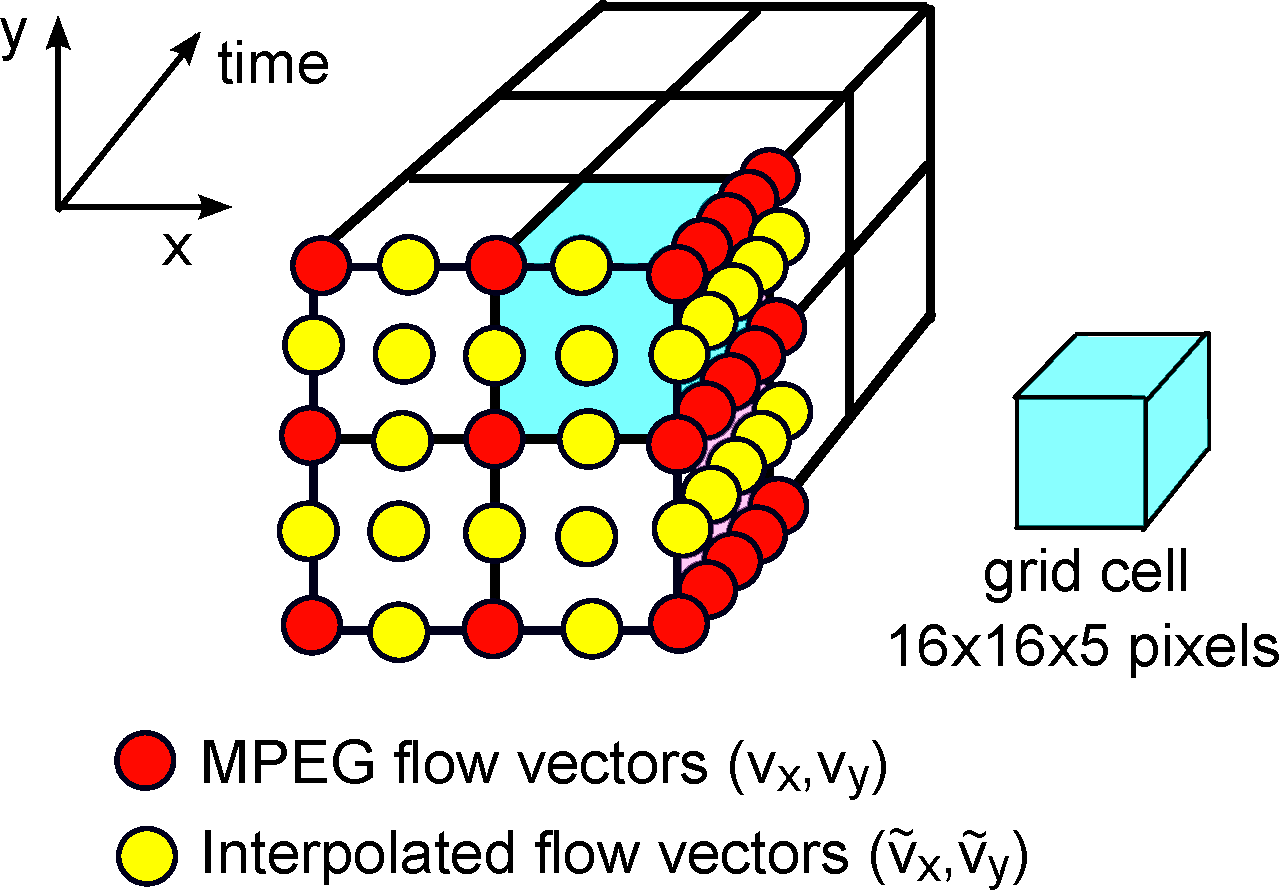
\includegraphics[width=.7\linewidth]{figures/CD-descriptor2.pdf}
\caption{The descriptor layout. Each $2\times2\times3$ descriptor cell is accumulated from quantized values of flow values.\vspace{-.7cm}}
\label{fig:CDdescriptor}
\end{center}
\end{figure}

We follow the design of previously proposed space-time
descriptors~\cite{Laptev08,Wang12} and define our descriptor by
histograms of flow vector orientations accumulated in a video patch. Each patch is divided into cells as illustrated in
Figure~\ref{fig:CDdescriptor} and the normalized histograms from
patch cells are concatenated into a descriptor vector.

Following~\cite{Wang12}, we compute HOF descriptors as
histograms of flow orientations discretized into eight orientation bins and a no-motion bin. For MBHx and MBHy descriptors the spatial
gradients of the $v_x$ and $v_y$ components of the flow are
similarly discretized into nine bins. 
The final descriptor is obtained by concatenating histograms
from each cell of the $2\times2\times3$ descriptor grid followed
by $l_2$-normalization of every temporal slice. HOG descriptors
are computed at the same set of points.

The temporal stride is fixed to 5 frames, while the spatial scale and sampling pattern are subject to tweaking in Subsection~\ref{subsec:sparse_opt_flow} and Subsection~\ref{subsec:sparse_mv_flow}. 

\subsection{Features from sparse flow}
\label{subsec:sparse_opt_flow}
Optical flow occupies a large portion of time in
descriptor computation. In order to achieve faster than
real-time
performance we evaluate a natural speed-up - estimating optical
flow
at a smaller point set.

\subsection{Efficient features from compressed video}
\label{subsec:sparse_mv_flow}
Motion vectors + figure... Evaluation on BOF/histograms on
UCF50/HMDB/HWD/UTI. Codecs, channels. Breakdown.

%The above scheme defines a $32\times32\times15$ pixel descriptor which we compute at every location of the video defined by the spatial stride of $16$ pixels and temporal stride of $5$ frames. To sample multiple spatial scales, we similarly define a $48\times48\times15$ pixel descriptor sampled with $24$ pixels spatial stride. For a video of $640\times480$ pixels spatial resolution we obtain around 300 descriptors per frame. This is comparable to $\approx350$ dense trajectory features produced by the method in~\cite{Wang12} for the same video resolution.

\subsection{Role of trajectories}
Discussion of V*/V0.


\section{Descriptor encoding}
\label{sec:quantization}
Overview of encoding methods.

%The purpose of descriptor encoding is to transform collections of local image or video descriptors $\left\{\textbf{x}_i\dots\textbf{x}_N\right\}$ into fixed-size vector representations.
%In this paper we investigate two descriptor encoding schemes and propose their computational improvements as described below.

%\subsection{Histogram encoding}
%\label{subsec:histenc}
%Histogram encoding is a common method for representing video by local descriptors. First, for each descriptor type (HOG, HOF, MBHx, MBHy) a vocabulary of $K$ visual words is constructed using the K-means algorithm. Then each descriptor is assigned to one of the visual words. Then the visual word indices are accumulated in a histogram. We follow~\cite{Laptev08} and use ``space-time pyramid'' which allows to capture the rough spatial and temporal layout of action elements. We split videos into six space-temporal grids ($x\times y \times t$: 1x1x1, 2x2x1, 1x3x1, 1x1x2, 2x2x2, 1x3x2x, in total 24 cells). In total we have $C=96\text{ channels} = 4 \text{ descriptor types}\times 24\text{ cells}$, that is one channel per a pair of descriptor type and grid cell. Each cell accumulates its own histogram which is then $l_1$-normalized, thus the total histogram representation size is $C\cdot K$. We also employ space-time pyramids for the Fisher vector and VLAD encoding methods.
%
%For assignment we experimented with using brute-force nearest neighbors and with using the kd-trees from the FLANN library. The motivation for using kd-trees is the significant improvement in processing speed over the brute-force algorithm (see Subsection~\ref{subsec:descencimprov}). The main parameters for the kd-trees method are the number of trees and the number of tests  made during the descent over the trees. 
%
%\subsection{Fisher vector}
%Fisher vector has been reported to consistently improve the performance for the image classification and image retrieval tasks~\cite{Jegou12}. Another advantage over the histogram encoding is that Fisher vectors allow the linear kernel classification. Fisher vector encoding assumes that descriptors are generated by a GMM model with diagonal covariance matrices. Similarly to histogram encoding, the GMM model of $K$ Gaussians is first learned on the training set. 
%Once the model $\left(\boldsymbol\mu_k, \boldsymbol\sigma_k\right)$ is learned, the Fisher vector representation of the descriptors $\left\{\textbf{x}_1\dots \textbf{x}_N\right\}$ is given by the two parts \cite{Perronnin10}:
%$${\textbf u}_k = \frac{1}{N\sqrt{\pi_k}}\sum_{i=1}^{N}q_{ki}\left(\frac{\textbf{x}_i-\boldsymbol\mu_k}{\boldsymbol\sigma_k}\right)$$
%
%\begin{equation}
%\label{eq:fv_vk}
%\textbf{v}_k=\frac{1}{N\sqrt{2\pi_k}}\sum_{i=1}^{N}q_{ki}\left[\left(\frac{\textbf{x}_i-\boldsymbol\mu_k}{\boldsymbol\sigma_k}\right)^2-\textbf{1}\right]
%\end{equation}
%where $q_{ki}$ is the Gaussian soft assignment of the descriptor $\textbf{x}_i$ to the $k$-th Gaussian, $\pi_k$ are the mixture weights, division and square are term-by-term operations. The \textbf{u} part captures the first-order differences, the \textbf{v} part captures the second-order differences. The final representation of size $C\cdot 2DK$ is given by concatenation of the two parts. As suggested by \cite{Perronnin10}, at the end we take signed square root and $l_2$-normalize the result. We apply the same normalization scheme to VLAD.
%\subsection{VLAD}
%The VLAD encoding is the simplified version of Fisher vector which considers only the first-order differences and assigns descriptors to a single mixture component. It was also shown to out-perform pure histogram encoding \cite{Jegou12}. In our variant we keep the soft-assignment factor $q_{ki}$. The VLAD representation of size $C\cdot DK$ is then given by concatenating:$$\textbf{u}_k=\sum_{i : NN\left(\textbf{x}_i\right)=\boldsymbol\mu_k}q_{ki}\left(\textbf{x}_i -\boldsymbol\mu_k\right)$$



\section{Experimental evaluation}
\label{sec:experiments}
Evaluation of VLAD / FV with different parameters. Breakdown.
Below is the copy over from the ICCV paper:



\begin{table*}[t!]
\begin{center}
\begin{tabular}{p{.65\textwidth}p{.32\textwidth}}
\hspace*{.4cm}
\begin{tabular}{|l||c|c||c|c|}
\hline
\multirow{3}{*}{} &\multicolumn{2}{c||}{Classification} & \multicolumn{2}{c|}{Speed}\\
                  &\multicolumn{2}{c||}{(mAP)} & \multicolumn{2}{c|}{(fps)}\\
\cline{2-5}
& CD (our) & DT~\cite{Wang12} & CD (our) & DT~\cite{Wang12}\\
\hline\hline
HOF               & 47.2\% & 52.9\% & 346.8 &  \\\hline
MBHx              & 49.0\% & 52.0\% & 330.3 &  \\\hline
MBHy              & 50.4\% & 56.1\% & 330.3 &  \\\hline
HOF+MBHx+MBHy     & 53.9\% & 58.9\% & 218.7 &  \\\hline
HOF+MBHx+MBHy+HOG & 56.2\% & 60.0\% & 168.4 & 1.2 \\\hline
\end{tabular}
&
\mbox{}\vspace{-.55cm}\newline
\hspace*{.2cm}
\begin{tabular}{|l|c|c|}
\hline
             & DivX  & x264  \\\hline
1024 kbit/s  & 54.3\% & 54.4\% \\\hline
512 kbit/s   & 54.5\% & 54.9\% \\\hline
256 kbit/s   & 54.2\% & 55.3\% \\\hline
128 kbit/s   & 53.4\% & 54.8\% \\\hline
\end{tabular}
%
%\begin{table}
%\begin{center}
%\begin{tabular}{|l|c|c|c|c|}
%\hline
%		&	128 kbit/s	&	256 kbit/s	&	512 kbit/s	&	1024 kbit/s 	\\\hline
%DivX	&	0.534			&	0.542			&	0.545			&	0.543				\\\hline
%x264	&	0.548			&	0.553			&	0.549			&	0.544				\\\hline
%\end{tabular}
%\caption{Evaluation of how video bitrate affects classification accuracy. All results were obtained by using FLANN kd(4)-ch(32) quantization.\vspace{-.3cm}}
%\label{tab:bitrates}
%\end{center}
%\end{table}
\end{tabular}
\mbox{}\vspace{.1cm}\\
\caption{{\bf Left:} Evaluation of action classification accuracy and the speed of feature computation for Hollywood2 action recognition benchmark. The speed of feature computation is reported for video of spatial resolution $640\times480$ evaluated on a single core Intel Xeon E5345 2.33Hz processor.
{\bf Right:} Evaluation of action recognition accuracy in Hollywood2 under the variation of video compression in terms of video codecs and compression bit-rates. The results are reported for CD descriptors in combination with histogram encoding.
\vspace{-.4cm}}
\label{tab:HWD2}
\end{center}
\end{table*}

%In this section we evaluate the proposed descriptor and descriptor encoding schemes on Hollywood2~\cite{Marszalek09} and UCF50~\cite{Reddy12} action recognition benchmarks and compare the speed and the recognition accuracy to the state of the art. We report classification results as mean average precision (mAP) for Hollywood2 and accuracy (Acc.) for UCF50. Processing speed is reported as frame-per-second (fps). We first evaluate the accuracy and the computational cost of proposed descriptor and compare it to the state-of-the-art method~\cite{Wang11}. The second part of the evaluation concerns the speed and accuracy of descriptor encoding.

In this section we evaluate the proposed descriptor and encoding schemes on Hollywood2~\cite{Marszalek09}, UCF50~\cite{Reddy12} and UT-Interaction~\cite{Ryoo10} action recognition benchmarks (see Figure~\ref{fig:datasets}) and compare the speed and accuracy of action recognition  to the state of the art. We report classification results as mean average precision (mAP) for Hollywood2 and mean accuracy (acc) for UCF50 and UT-Interaction datasets. The processing speed is reported in frames-per-second (fps). We first evaluate the accuracy and the computational cost of the proposed descriptor and compare results with~\cite{Wang12}. We then evaluate the speed, accuracy and compression of descriptor encoding.

%In this series of experiments we adopt the standard bag-of-features action classification pipeline~\cite{Schuldt04} and represent each video clip by a $l_1$-normalized histogram of quantized local features. For each extracted type of descriptor we compute a vocabulary of 4000 visual words using k-means and assign all features to their nearest visual word centroids. Taking into account the space-time pyramid, we end up with $4\times24=96$ channels which we put in the SVM with multi-channel exponential $\chi^2$-kernel~\cite{Zhang07}.

To recognize actions we use SVM with multi-channel exponential $\chi^2$-kernel~\cite{Zhang07} together with histogram-based action representations. For Fisher vector and VLAD encodings we use linear SVMs.


\subsection{Descriptor evaluation}
%To assess the performance of motion information in compressed video representation, we first evaluate the performance of STIP features~\cite{Laptev08} where MPEG flow was obtained from DivX compression of Hollywood2 video samples and upscaled to the original video resolution. Results for one channel HOF descriptors in this setup gives 0.432 mAP compared to 0.458 mAP obtained for the original STIP implementation using Lucas-Kanade optical flow.

Table~\ref{tab:HWD2}(Left) presents results of action recognition using the proposed compressed domain (CD) features %described in Section~\ref{sec:CDdescriptor} 
and compares performance to Dense Trajectories (DT) baseline~\cite{Wang12}. For the full combination of four descriptors the performance of DT (60.0\%) is approximately four per-cent higher compared to CD features (56.2\%). When comparing the speed of feature extraction for both methods measured on videos with $640\times480$ pixels spatial resolution, our method achieves 168fps which is about 7 times faster than real-time and 140 times faster compared to~\cite{Wang12}. The speed measurements in this experiment include the time of feature computation as well as the time for video reading and decompression. Most of the time for our method is spent on the computation of integral histograms and aggregation of histogram-based video descriptors. Reducing the number of descriptor types increases the speed of our method to 347fps (14 times real time) at the cost of 9\% drop in mAP.

%We also evaluate how the codec used for encoding and video bitrate affect the classification accuracy on the Hollywood2 dataset. The results are available in Table~\ref{tab:bitrates}. One can note there is no significant difference between motion estimates of x264 and DivX 5.2.1 (both with standard profile). In addition, one can see that accuracy does not drastically decrease w.r.t. bitrate, which allows to encode video with low bitrate if action recognition is the eventual purpose. We used FLANN kd(4) + checks(32) as the quantization method for this experiment.

DT features~\cite{Wang12} are computed along point tracks which is different to our features computed inside the fixed-size video patches. To identify the reason for 4\% mAP drop of our method compared to~\cite{Wang12} we simplify DT features by first approximating free-shape trajectories in DT features by straight lines (DT V*). In the second simplification we remove trajectory information from DT descriptor and compute DT features in fixed axes-parallel cuboids (DT V0). The results of these modifications in the first two lines of Table~\ref{tab:HWD2traj} indicate 1\% drop due to DT V* and 1\% further drop in mAP due to DT V0. Explicitly including the shape of trajectories into the descriptor (last line of Table~\ref{tab:HWD2traj}) does not improve performance significantly. From this experiment we conclude that the shape of trajectories does not contribute to other descriptors significantly. We believe that the difference in accuracy of DT features and our method should be in the denser and more accurate flow estimation deployed by DT. Per-class action classification comparison of CD and DT features is illustrated in Figure~\ref{fig:hwd2-barplot}.

MPEG flow might be influenced by the types and parameters of video codecs. To investigate this aspect, we evaluate the performance of action recognition for two common video codecs (x264 and DivX 5.2.1) under varying video compression bit-rates. Results in Table~\ref{tab:HWD2}(Right) indicate the stable performance of action recognition for different types of video codecs and decreasing video quality corresponding to low values of bit-rates.

\begin{table}
\begin{center}
\begin{tabular}{|l|c|c|}
\hline
& mAP \\\hline
HOF+MBHx+MBHy+HOG (V0)  					& 58.0\%	\\\hline
HOF+MBHx+MBHy+HOG (V*)						& 58.9\%	\\\hline
HOF+MBHx+MBHy+HOG \cite{Wang12}     	& 60.0\% 	\\\hline
HOF+MBHX+MBHY+HOG+TRAJ \cite{Wang12} 	& 60.3\% 	\\\hline
\end{tabular}
\mbox{}\vspace{.2cm}\\
\caption{Action classification accuracy for different versions of the dense trajectory features~\cite{Wang12}.\vspace{-.7cm}}
\label{tab:HWD2traj}
\end{center}
\end{table}



\subsection{Descriptor encoding evaluation}
\label{subsec:descencimprov}
While our method achieves high speed descriptor computation, the feature quantization becomes a bottle-neck with nearest-neighbor (NN) quantization performing only at the rate of 10fps when using efficient $l_2$-distance implementation. To improve quantization speed, we experiment with tree-based approximate nearest neighbor (ANN) quantization schemes implemented in FLANN~\cite{Muja09}. The trade-off between computational time and the accuracy of quantization measured on the final recognition task is illustrated in Figure~\ref{fig:hwd2-flann}. Notably, the quantization using four trees and 32 tests in ANN search does not degrade recognition performance and achieves factor $\approx5$ speed-up compared to NN. Further increase of the speed implies approximately linear degradation of classification accuracy. 

We next investigated Fisher Vector (FV)~\cite{Perronnin12} and VLAD encodings~\cite{Jegou10} described in Section~\ref{sec:quantization}. 
%FV and VLAD representations have been shown to achieve high accuracy for image classification tasks~\cite{Chatfield11} and usually require smaller vocabularies compared to histogram encodings.
%
%Fisher vector and VLAD schemes are described in Section~\ref{sec:quantization}. 
To the best of our knowledge, Fisher vector and VLAD encodings have not been applied to action classification earlier. We train a GMM model with $K=256$ Gaussians \cite{Jegou12}. Results in Figure~\ref{fig:hwd2-flann} and Table~\ref{tab:hwd2_comparison} indicate improvements in both the speed and accuracy when using FV and VLAD encodings compared to the histogram encoding. As for the histogram encoding, FLANN provides considerable speed-up for FV and VLAD encodings.

Table~\ref{tab:ucf_comparison} presents action recognition results for the UCF50 dataset. Similar to the Hollywood-2 dataset, the accuracy of our methods is only a few percent below the state-of-the-art results in~\cite{Wang12} with FV and VLAD encodings providing improvements over the histogram encoding both in speed and accuracy. The overall speed improves the speed of~\cite{Wang12} by two orders of magnitude. Table~\ref{tab:uti_comparison} presents results for the UT-Interaction dataset and compares our method with the efficient action recognition method~\cite{Yu10}. Our method demonstrate better classification accuracy compared to~\cite{Yu10} and improves the speed of~\cite{Yu10} by the factor of $10$.

%Our Fisher vector implementation attributes a descriptor only to 5 nearest mixture centroids in $l_2$-sense in contrast to \cite{Jegou12} which fully computes $q_{ki}$ to all mixture centroids in their public implementation in the YAEL library\footnote{\scriptsize \url{https://gforge.inria.fr/projects/yael/}}. To make it faster we compute only the 5 nearest neighbors using kd-trees. Differently from YAEL we explicitly tailor our implementation to efficiently compute Fisher vector for several spatio-temporal grids. In addition, we found that the second order part $\textbf{v}_k$ (\ref{eq:fv_vk}) does not bring improvement, and we don't compute it.

%We also experiment with the VLAD representation that we get if we consider only one nearest neighbor during the process described above. With both representations we try different values for the number of tests performed during the descent down the kd-trees.

\begin{figure}
\begin{center}
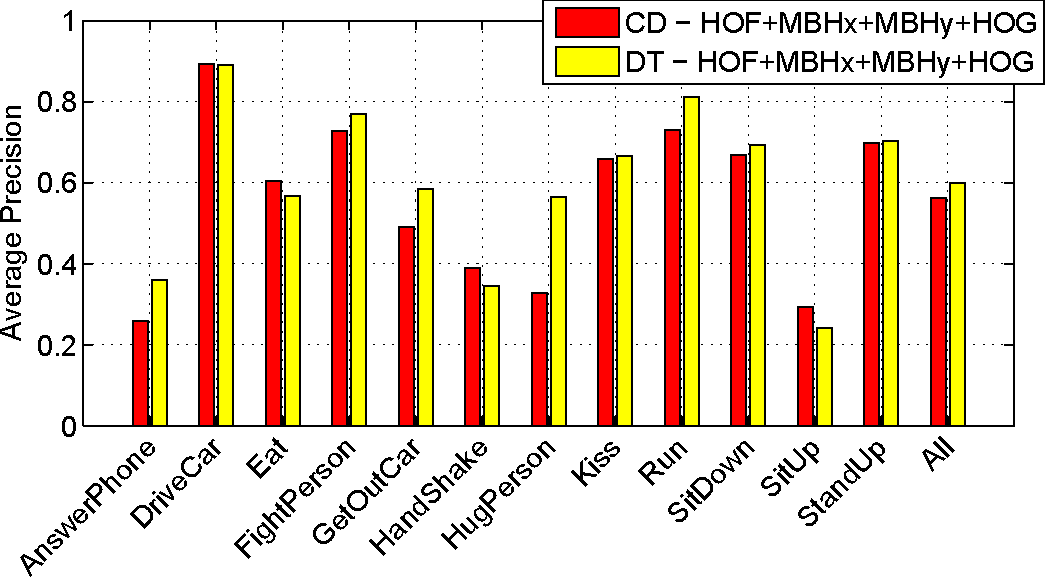
\includegraphics[width=.9\linewidth]{figures/hollywood2-per-class-barplot-crop.pdf}.
\caption{Per-class action classification results for DT~\cite{Wang12} and our  CD features using HOF+MBHx+MBHy+HOG descriptor combination and histogram encoding on the Hollywood2 benchmark.\vspace{-.1cm}}
\label{fig:hwd2-barplot}
\end{center}
\end{figure}

\begin{figure}
\begin{center}
\mbox{}\vspace{-.4cm}\\
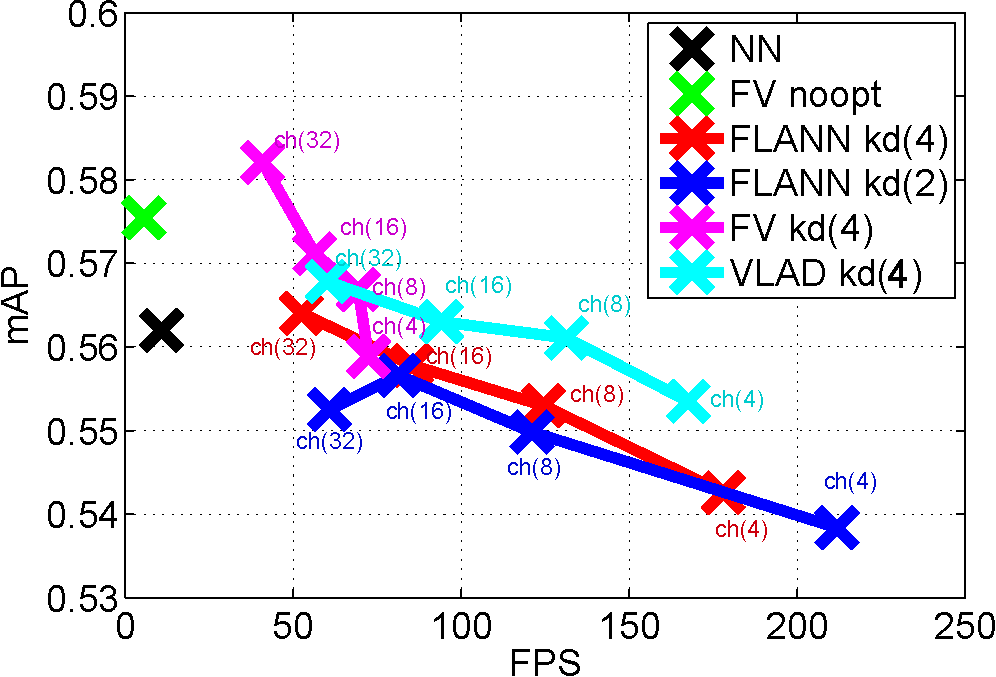
\includegraphics[width=.9\linewidth]{figures/hollywood2-flann-fps-map-crop-mod.pdf}
\caption{Performance of action recognition and the speed of descriptor encodings in Hollywood2 dataset for different types and parameters of encoding schemes. kd($x$) indicates the number of trees $x$ in the kd-forest used for ANN descriptor assignment. ch($y$) indicates the number of tests $y$ when descending the forest.\vspace{-.4cm}}
\label{fig:hwd2-flann}
\end{center}
\end{figure}


%\begin{table}
%\begin{center}
%\begin{tabular}{|l|c|c|}
%\hline
%& Classification & Speed\\
%& (mAP) & (fps)\\\hline
%Nearest Neighbour    & 0.562 &  10.8 \\\hline
%FLANN kd(4)-ch(32)   & 0.564 &  52.3 \\\hline
%FLANN kd(4)-ch(16)   & 0.558 &  85.2 \\\hline
%FLANN kd(4)-ch(8)    & 0.553 & 124.5 \\\hline
%FLANN kd(4)-ch(4)    & 0.542 & 177.9 \\\hline
%FLANN kd(2)-ch(16)   & 0.556 &  81.3 \\\hline
%FLANN kd(2)-ch(8)    & 0.550 & 121.0 \\\hline
%FLANN kd(2)-ch(4)    & 0.538 & 211.8 \\\hline
%\end{tabular}
%\caption{Evaluation of feature quantization using exact nearest neighbour and different variants of kd-tree based approximate nearest neighbour~\cite{Muja09}.\vspace{-.3cm}}
%\label{tab:quantization}
%\end{center}
%\end{table}

%\begin{table}
%\begin{center}
%\begin{tabular}{|l|c|c|}
%\hline
%					& HWD2		& UCF50 		\\\hline  % & HMDB51
%FLANN(4-32) 	& 55.88	& 81.62\% 	\\\hline % & 39.803922	
%VLAD(4)			& 56.78 & 80.65\% 	\\\hline % & 36.535948	
%FV(32) 			& 58.21	& 82.25\% 	\\\hline % & 37.450981	
%\end{tabular}
%\caption{Evaluation of how descriptor encoding method affects classification accuracy.\vspace{-.3cm}}
%\label{tab:quantization_comparison}
%\end{center}
%\end{table}

\begin{table}
\begin{center}
\begin{tabular}{|l|c|c|c|c|}
\hline
		 				&  	 		& Feat.                   	& Quant. 		& Total		\\
		 				& Acc.  	& (fps)								& (fps)			& (fps)		\\\hline
CD FLANN(4-32)	& 55.8\%	& \multirow{3}{*}{168.4} 	& 52.4    	& 40.0 	\\ % FPS = 1/(1/168.4 + 1/52.3921)
CD VLAD(4) 		& 56.7\%	&										& 167.5	& 84.0	\\ % FPS = 1/(1/168.4 + 1/167.537313)
CD FV(32)			& 58.2\%	&										& 40.9 	& 32.9	\\ % FPS = 1/(1/168.4 + 1/40.8925322)
\hline
DT \cite{Wang12}& 59.9\%		& 1.2									& 5.1 		&	1.0	\\\hline % Quant. FPS = 1346 frames / 266.17 secs = 5.0569 FPS; Total = 1/(1/1.2 + 1/5.0569) = 0.9699 FPS
%\cite{le_at_al}						& 53.3\%		&										&				&\\\hline
\end{tabular}
\mbox{}\\
\caption{Comparison of our method to the state of the art on Hollywood2 dataset. The speed of~\cite{Wang12} and of our method is reported for videos with $640\times 480$ spatial resolution using the same single core Intel Xeon E5345 2.33Hz processor.\vspace{-.3cm}}
\label{tab:hwd2_comparison}
\end{center}
\end{table}



\begin{table}
\begin{center}
\begin{tabular}{|l|c|c|c|c|}
\hline
		 				&  	 	& Feat.                    & Quant. 	& Total	\\
		 				& Acc.  & (fps)                    & (fps) 	& (fps)	\\\hline
CD FLANN(4-32)	& 81.6\% & \multirow{3}{*}{591.8}   & 52.4  	& 48.1	\\ % FPS = 1/(1/592 + 1/52.3921)
CD VLAD(4) 	 	& 80.6\% &                          & 671.4 	& 314.6	\\ % FPS = 1/(1/592 + 1/671.428571)
CD FV(32)	 		& 82.2\% &                          & 171.3 	& 132.8	\\ % FPS = 1/(1/592 + 1/171.255061)
\hline
DT \cite{Wang12}& 85.6\% & 2.8            	        & 5.1  	& 1.8\\\hline%  Feat extr FPS = 846 frames / 5m; Quant FPS = 846 frames / 166.17 secs = 5.0912 FPS; Total = 1 / (1/2.8 + 1/5.0912) = 1.8065 FPS
%\cite{Kliper12}		&	72.7\%	&									&			&\\\hline
\end{tabular}
\smallskip
\caption{Comparison of our method to the state of the art on the UCF50 dataset~\cite{Reddy12}. The speed is reported for videos with the spatial resolution $320\times 240$ pixels.}
\label{tab:ucf_comparison}
\mbox{}\vspace{-1cm}\\
\end{center}
\end{table}


\begin{table}
\begin{center}
\begin{tabular}{|l|c|c|}
% set1_segmented
%   sample acc = 85.238095
%   feat extr fps = 7280 frames / 15.990000 sec = 455.2846 fps
%	 quant time fps = 7280 frames / 61.720000 = 117.9520 fps
%   total_fps = 1 / (1/455.2846 + 1/117.9520) = 93.6816 fps
% set2_segmented
%	 sample acc = 87.6190
% 	 feat extr fps = 6515 frames / 12.160000 sec = 535.7730 fps
%   quant time fps = 6515 frames / 50.100000 = 130.0399fps
%   total_fps = 1 / (1/535.7730 + 1/130.0399) = 104.6418
% average fps: (93.6816 + 104.6418)/2 = 99.1617
% average acc: (85.238095 + 90.000000) / 2 = 87.6190
\hline
								& Acc.		& Total FPS	\\\hline
FV(32)						& 87.6\%		& 99.2		\\\hline
PSRM+BOST\cite{Yu10}	& 83.3\%		& 10.0 		\\\hline

\end{tabular}
\mbox{}\vspace{.2cm}\\
\caption{Accuracy and speed of action recognition in the UT-interaction dataset~\cite{Ryoo10}.\vspace{-.6cm}}
\label{tab:uti_comparison}
\end{center}
\end{table}

\begin{figure}
\begin{center}
%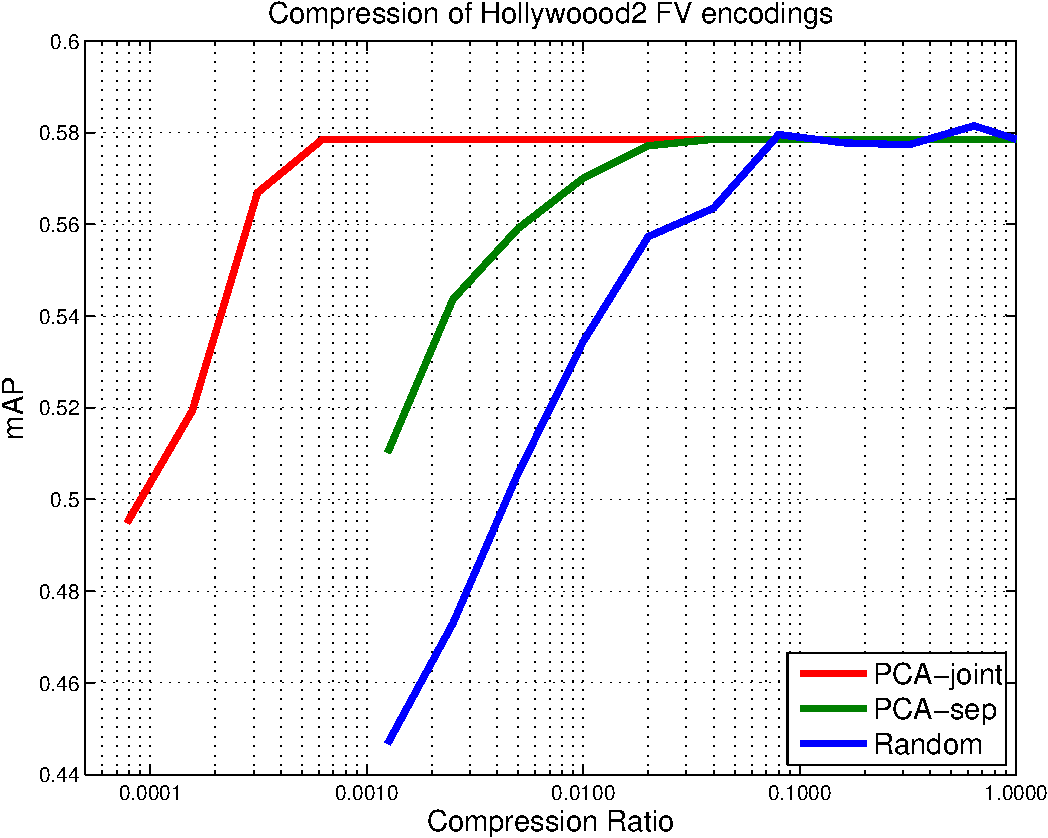
\includegraphics[width=.8\linewidth]{figures/compression/compression-hwd2-FV-sum96-cropped.pdf}
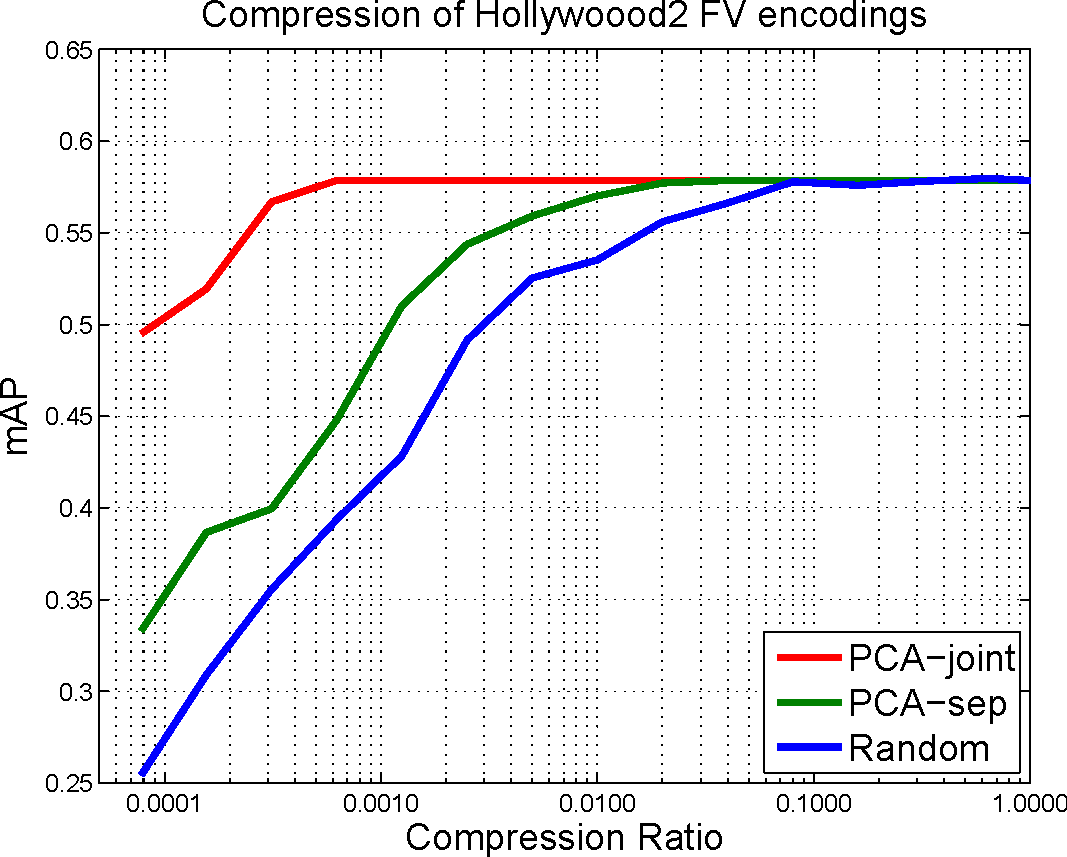
\includegraphics[width=.8\linewidth]{figures/compression/compression-hwd2-FV-sum96-all-cropped.pdf}
\caption{Action recognition results on the Hollywoood-2 dataset using compressed FV encoding.\vspace{-.5cm}}
\label{fig:dimred}
\end{center}
\end{figure}



%Hollywood2 results (A): Compressed domain features
%HOF: 0.472243
%MBHx: 0.490259
%MBHy: 0.503737
%HOF+MBHx+MBHy: 0.539212
%HOF+MBHx+MBHy+HOG (m/channel): 0.561959
%HOF+MBHx+MBHy+HOG (single vocab): 0.517230

%Hollywood2 results (B): Dense trajectory features
%HOF : 0.528732
%MBHX : 0.519922
%MBHY : 0.561268
%HOF_MBHX_MBHY : 0.589344
%HOF_MBHX_MBHY_HOG : 0.599716
%HOF_MBHX_MBHY_TRAJ : 0.591272
%HOF_MBHX_MBHY_HOG_TRAJ: 0.603235

%HOG+HOF+MBHx+MBHy:
%VEL0: 0.580140
%FST: 0.589389

%Hollywood2 results (C): Compressed domain features + FLANN; 
%HOF: 0.480621
%MBHx: 0.480726
%MBHy: 0.499320
%HOF+MBHx+MBHy: 0.540788
%HOF_MBHx_MBHy_HOG (m/channel): 0.564032

% per-class results in 
% https://docs.google.com/spreadsheet/ccc?key=0Al7q11u9-vugdDk4UlhrWjVxNm5Ldk9EMjVEZTZVM0E&pli=1#gid=0
% D:\doc\papers\descriptors\cvpr13\results\Class. results by class.xlsx

%%%%%%%%%%% computation time, election video 1800 frames 120 sec. 15fps (-> 72sec at 25fps)
% CD features   10.69 sec ->  168.3817 fps
% HOF only:     5.19 sec -> 346.8 fps
% MBHx 0nly:    5.45 sec -> 330.3 fps
% HOF+MBHx+MBHy 8.23 sec -> 218.7 fps
%
%# STAT. Descriptor computation: 3.13 secs
%# STAT. HOF: 0.42, MBH: 1.49 secs, HOG: 0.71 secs
%# STAT. Interpolation. HOFMBH: 0.14 secs, HOG: 0.37 secs
%# STAT. Descriptor querying: 3.60 secs
%# STAT. HOF: 0.84, MBH: 1.55 secs, HOG: 0.79 secs
%# STAT. Reading: 0.04 secs
%# STAT. Decoding: 3.75 secs
%# STAT. Writing: 87.96 secs
%# STAT. ---
%# STAT. Total: 98.65 secs
%# STAT. fps: 18.24
%# STAT. calls:
%# STAT. --ComputeDescriptor     6467808
%
% DT features: 24m56sec -> 1.2032 fps
%
% CD vs. DT speedup: x139.9449

%%%%%%%%%%% computation time, actioncliptest00775 1347 frames, 53.8 sec.
% CD features 9.35 sec -> 144.0642 fps
%# STAT. Descriptor computation: 2.79 secs
%# STAT. HOF: 0.29, MBH: 1.28 secs, HOG: 0.85 secs
%# STAT. Interpolation. HOFMBH: 0.07 secs, HOG: 0.30 secs
%# STAT. Descriptor querying: 3.22 secs
%# STAT. HOF: 1.00, MBH: 1.27 secs, HOG: 0.61 secs
%# STAT. Reading: 0.04 secs
%# STAT. Decoding: 3.00 secs
%# STAT. Writing: 71.45 secs
%# STAT. ---
%# STAT. Total: 80.80 secs
%# STAT. fps: 16.67
%# STAT. calls:
%# STAT. --ComputeDescriptor     4596504
%
% DT features 28m37sec -> 0.7845 fps
% real    28m37.449s
% user    28m26.158s
% sys     0m13.664s
%
% CD vs. DT speedup: x183.6382



% Quantization for actioncliptest00775 1347 frames, 53.8 sec.
%
%
% kd(8) + checks(32) 38.90 secs ->  34.6272      mAP 0.563959
% kd(8) + checks(16) 23.56 secs ->  57.1732      mAP 0.560811
% kd(8) + checks(8)  13.18 secs -> 102.2003      mAP 0.553482
% kd(8) + checks(4)  11.52 secs -> 116.9271      mAP 0.526568

% kd(4) + checks(32) 25.71 secs ->  52.3921 fps (mAP 0.564032)

% kd(4) + checks(16) 15.80 secs ->  85.2532     (mAP 0.557820)
% kd(4) + checks(8)  10.82 secs -> 124.4917     (mAP 0.552988)
% kd(4) + checks(4)   7.57 secs -> 177.9392     (mAP 0.542571)
% kd(2) + checks(32) 22.17 secs ->  60.7578     (mAP 0.552528)
% kd(2) + checks(16) 16.56 secs ->  81.3406     (mAP 0.556588)
% kd(2) + checks(8)  11.13 secs -> 121.0243     (mAP 0.549832)
% kd(2) + checks(4)   6.36 secs -> 211.7925     (mAP 0.538391)
%
%

%Quantization for actioncliptest00775 1347 frames, regular FV, just mu params
%Options:
%Indices are zero-based
%213-308 '../../vocab/mbhx_K256.vocab'
%Build GMM index: no
%GMM components: 256
%Lambda reg: 0.000000
%Output file path: out.npy
%Zero all gamma but: 0
%XnPos: 0, YnPos: 1, TnPos: 2
%Grids: 1x1x1x
%Vocabularies loaded
%
%#FV 1x1x1x  mbhx_K256 (213-308)
%fts.cols: 96
%24576
%No zeroing
%24576
%# 0-0-0 (380014)
%#STAT Vocab reading and construction: 0.03 secs
%#STAT Reading: 21.32 secs
%#STAT Writing: 0.00 secs
%#STAT Assigning: 164.76 secs
%#STAT Copying: 0.41 secs
%#STAT Total: 186.54 secs
%#STAT Ops: 1
%#STAT Descriptors: 380014
%#STAT Part sizes: 96

% Quantization for actioncliptest00775 w=640	h=480	frames=1347.00
%KNN_TREES_CHECKS FLANN ASSIGNING TOTAL FPS
%5_4_32 22.870000 10.070000 32.940000 40.892532		mAP 0.582075 (c =1e-3)
%5_4_16 13.890000 9.990000 23.880000 56.407035		mAP 0.571156 (c=1)
%5_4_8 9.000000 10.430000 19.430000 69.325785		mAP 0.566866 (c=1)
%5_4_4 6.720000 11.880000 18.600000 72.419355		mAP 0.558892 (c=1)

%1_4_32 19.780000 2.650000 22.430000 60.053500		mAP 0.567833 (c=1)
%1_4_16 11.580000 2.730000 14.310000 94.129979		mAP 0.563006 (c=0.1-1)
%1_4_8 7.540000 2.720000 10.260000 131.286550		mAP 0.561079 (c=1)
%1_4_4 5.300000 2.740000 8.040000 167.537313			mAP 0.553502 (c=1)

%3_4_32  21.350000       6.300000        27.650000       48.716094 mAP 0.565615 (c=1)
%3_4_16 mAP 0.562545 (c=1e-1)
%3_4_8 mAP 0.565996 (c=1)
%3_4_4   5.730000        6.760000        12.490000       107.846277 mAP 0.558180 (c=1)



%UCF50 w=320	h=240 frames=846.00 v_Rowing_g15_c05.avi  ; #features: 48944 => 57.8 features / frame
%5_4_32  3.350000        1.590000        4.940000        171.255061
%1_4_4   0.810000        0.450000        1.260000        671.428571
% feature extraction:  1.4200 => 595.7746 fps
%5_4_32 => total fps: 132.8761
%1_4_4  => total fps: 315.6401


%HMDB51 w=320 h=240	frames=75.0 Iaido_video_instruction_series_Wehrhahn_Sensei_sword_exercise_f_nm_np1_le_bad_1.avi  ; #features: 3864 => 51.5 features / frame
%5_4_32  0.300000        0.110000        0.410000        182.926829
%1_4_4   0.060000        0.040000        0.100000        750.000000
% feature extraction: 0.18sec => 416.6667 fps
%5_4_32 => total fps: 127.0918
%1_4_4  => total fps: 267.5815

%UCF50 extr. time on v_Rowing_g15_c05.avi. !! DescrComp + Interp + DescrQue + Reading + Decoding: 1.43 sec, 846 frames => 592 fps 
%# STAT. Descriptor computation: 0.47 secs
%# STAT. HOF: 0.05, MBH: 0.21 secs, HOG: 0.15 secs
%# STAT. Interpolation. HOFMBH: 0.01 secs, HOG: 0.05 secs
%# STAT. Descriptor querying: 0.55 secs
%# STAT. HOF: 0.13, MBH: 0.25 secs, HOG: 0.07 secs
%# STAT. Reading: 0.01 secs
%# STAT. Decoding: 0.34 secs
%# STAT. Writing: 8.97 secs


\subsection{Dimensionality reduction}
\label{sec:dimredexp}
We evaluate PCA dimensionality reduction of FV encoding on the task of action recognition in the Hollywood-2 dataset. Figure~\ref{fig:dimred} and Table~\ref{tab:compression} illustre recognition accuracy as a function of compression ratios and PCA compression methods as described in Section~\ref{sec:dimred}. Together with PCA-sep and PCA-joint methods we test a naive compression by removing elements of the FV representation at random. PCA-joint method indicates reduction of FV size from 2,4M elements to 1.5K elements without affecting the recognition performance.

%randomly removing eleselecting   shows the results of the first stage of the compression where we compress every cell separately. We found that without any affect to mAP we can take as few as 4\% of the ransformed coordinates. The results are shown in Figure~\ref{fig:dimred}.


%--------------------------------------------------- Results compression:
%
%-- PCA-joint --
%      190       380       760      1521      3041      6083     12165     24330     48660     97321 
% 0.000078  0.000156  0.000313  0.000625  0.001250  0.002500  0.005000  0.010000  0.020000  0.040000 
% 0.494944  0.519329  0.566903  0.578546  0.578546  0.578546  0.578546  0.578546  0.578546  0.578546 
%
%-- PCA-sep --
%       95       190       380       760      1521      3041      6083     12165     24330     48660     97321    194642    389284    778568   1557135   2433024 
% 0.000039  0.000078  0.000156  0.000313  0.000625  0.001250  0.002500  0.005000  0.010000  0.020000  0.040000  0.080000  0.160000  0.320000  0.640000  1.000000 
% 0.279528  0.332989  0.386662  0.399561  0.447897  0.510229  0.543665  0.559099  0.570052  0.577119  0.578548  0.578548  0.578548  0.578548  0.578548  0.578548 
%
%-- Random --
%       95       190       380       760      1521      3041      6083     12165     24330     48660     97321    194642    389284    778568   1557135   2433024 
% 0.000039  0.000078  0.000156  0.000313  0.000625  0.001250  0.002500  0.005000  0.010000  0.020000  0.040000  0.080000  0.160000  0.320000  0.640000  1.000000 
% 0.246643  0.254264  0.308998  0.355695  0.393686  0.428335  0.491417  0.525306  0.535146  0.556032  0.566180  0.577752  0.575865  0.578052  0.579643  0.578548 

%
%-- PCA-joint --
%      190       380       760      1521      3041      6083     12165     24330     48660     97321 
%99.992188 99.984375 99.968750 99.937500 99.875000 99.750000 99.500000 99.000000 98.000000 96.000000 
% 0.494944  0.519329  0.566903  0.578546  0.578546  0.578546  0.578546  0.578546  0.578546  0.578546 
%
%-- PCA-sep --
%     3041      6083     12165     24330     48660     97321    194642    389284    778568   1557135   2433024 
%99.875000 99.750000 99.500000 99.000000 98.000000 96.000000 92.000000 84.000000 68.000000 36.000000  0.000000 
% 0.510229  0.543665  0.559099  0.570052  0.577119  0.578548  0.578548  0.578548  0.578548  0.578548  0.578548 
%
%-- Random --
%     3041      6083     12165     24330     48660     97321    194642    389284    778568   1557135   2433024 
%99.875000 99.750000 99.500000 99.000000 98.000000 96.000000 92.000000 84.000000 68.000000 36.000000  0.000000 
% 0.446784  0.473019  0.505722  0.534434  0.557318  0.563524  0.579592  0.577746  0.577349  0.581466  0.578548 

\begin{table}
\begin{center}
\begin{tabular}{|l|c|c|c|c|}
\hline
Comp. ratio             &  0.00008  &     0.00063 &          0.04 &          1.0 \\\hline
Descr. size             &       190 &         1521 &         97321 &      2433024 \\\hline\hline
PCA-joint         &     49.4\% &        57.8\% &         57.8\% &        57.8\% \\\hline
PCA-sep           &     33.2\% &        44.7\% &         57.8\% &        57.8\% \\\hline
Random            &     25.4\% &        39.3\% &         56.6\% &        57.8\% \\\hline
\end{tabular}
\vspace{.0cm}%\smallskip
\caption{FV sizes and recognition accuracy on the Hollywood-2 dataset for different compression methods and ratios.\vspace{-.6cm}}
\label{tab:compression}
\end{center}
\end{table}


%\begin{table}
%\begin{center}
%\begin{tabular}{|l|c|c|c|c|}
%\hline
%Dimension	&	PCA-sep	 	&	PCA-joint	&	Random		\\\hline
%2433024		&	57.85\%	&					&	57.85\%	\\\hline
%1557135		&	57.85\%	&					&	58.15\%	\\\hline
%778568		&	57.85\%	&					&	57.73\%	\\\hline
%389284		&	57.85\%	&					&	57.77\%	\\\hline
%194642		&	57.85\%	&					&	57.96\%	\\\hline
%97321			&	57.85\%	&	57.85\%	&	56.35\%	\\\hline
%48660			&	57.71\%	&	57.85\%	&	55.73\%	\\\hline
%24330			&	57.01\%&	57.85\%	&	53.44\%	\\\hline
%12165			&	55.91\%&	57.85\%	&	50.57\%	\\\hline
%6083			&	54.37\%&	57.85\%	&	47.30\%	\\\hline
%3041			&	51.02\%&	57.85\%	&	44.68\%	\\\hline
%1521			&				&	57.85\%	&					\\\hline
%760			&				&	56.69\%	&					\\\hline
%380			&				&	51.93\%	&					\\\hline
%190			&				&	49.49\%	&					\\\hline
%\end{tabular}
%\smallskip
%\caption{PCA compression\vspace{-.3cm}}
%\label{tab:compression}
%\end{center}
%\end{table}



%%%%%%%%%%%%%%%%%%%%%%%%%%%%%%%%%%%%%%%%%%%%%%%%%%%%%%%%%%%%%%%%
%%%%%%%%%%%%% Conclusions
%%%%%%%%%%%%%%%%%%%%%%%%%%%%%%%%%%%%%%%%%%%%%%%%%%%%%%%%%%%%%%%%
\section{Conclusions}
We present an efficient method for extracting and encoding local descriptors in video. We show that sparse motion vectors from video compression enable accurate action recognition at reduced computational cost. We next apply and evaluate Fisher vector encoding for action recognition and demonstrate the improved speed and accuracy.
%Our efficient implementation of Fisher vector encoding, taking explicit care of space-time pyramids and selecting mixture components with FLANN, boosts accuracy and runs as fast as conventional histogram encoding with FLANN. 
We also address the problem of high dimensionality of Fisher vector signatures, and show drastic improvements in the size of FV using PCA. 
Out method is fast and enables accurate action recognition using small signatures and linear classifiers.

%evaluate applicability of PCA and present the scheme that compresses Fisher vector signatures from $2.5M$ to $1.5K$ ($\sim1000x$) values. Linear kernel is a natural choice for Fisher vectors\cite{Sanchez13} which makes classification instant. Particular variants of our system (like VLAD) run $\sim100$ faster than \cite{Wang11} and open doors to video analysis at larger scale.





{
\small
\bibliographystyle{cvpr2014authorKit_latex/ieee}
\bibliography{shortstrings,cvpr14}
}

\end{document}
